\begin{definition}[Sequences of Functions] \leavevmode \\
    Let $A \neq \empty$. If $\forall n \in \N$ we have $f_n: A \to \R,$ then
    $$f_1, f_2, f_3, ...$$
    is a sequence of functions and is denoted
    $$(f_n)_{n \geq 1}, (f_n), \text{ or } (f_n: A \to \R)_{n \geq 1}.$$
\end{definition}

\begin{example}
    \begin{enumerate}
        \item $(f_n)_{n\geq 1} = \left(\frac{\sin(nx)}{n}\right)_{n\geq 1}$ on the set $\R$:
        \begin{align*}
            f_1:\R \to \R, &f_1(x) = \sin x \\
            f_2:\R \to \R, &f_2(x) = \frac{1}{2}\sin 2x \\
            f_3:\R \to \R, &f_3(x) = \frac{1}{3}\sin 3x \\
            \vdots
        \end{align*}

        \item $(f_n)_{n\geq 1} = (x^n)$ on the set $[0,1]$:
        \begin{align*}
            f_1:[0,1] \to \R, &f_1(x) = x \\
            f_2:[0,1] \to \R, &f_2(x) = x^2 \\
            f_3:[0,1] \to \R, &f_3(x) = x^3 \\
            \vdots
        \end{align*}
        \begin{center}
            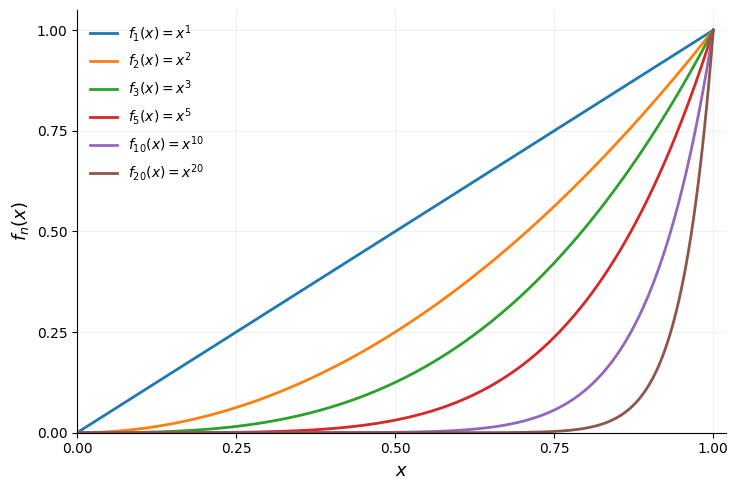
\includegraphics[width=0.5\textwidth]{CH7/images/Sequence of Functions [0,1].png}           
        \end{center}

        \item Let $f:[0,1] \to \R$ be a given function. For all $n \in \N$, let $f_n(x) = f(x^n)$. Then $(f_n)$ is a sequence of functions.
    \end{enumerate}
\end{example}

\begin{remark}
    Suppose $(f_n : A \to \R)_{n\geq 1}$ is a sequence of functions. Note that for each point $c \in A$, $(f_n(c)){n \geq 1}$ will be a sequence of numbers. For example, consider $(f_n(x) = x^n)_{n\geq 1}$ on the set $A = [0,2]$:
    \begin{align*}
        x=0: ~~~&f_1(0) = 0, f_2(0) = 0, f_3(0) = 0, ... \text{ is a sequence of numbers} \\
        x=1: ~~~&f_1\left(\frac{1}{2}\right) = \frac{1}{2}, f_2\left(\frac{1}{2}\right) = \frac{1}{2^2}, f_3\left(\frac{1}{2}\right) = \frac{1}{2^3}, ... \text{ is a sequence of numbers} \\
        x=2: ~~~&f_1(1) = 1, f_2(1) = 1, f_3(1) = 1, ... \text{ is a sequence of numbers} \\
        \vdots
    \end{align*}
\end{remark}

\begin{definition}[Pointwise Convergent Sequence] \leavevmode \\
    We say a sequence of functions $(f_n: A \to \R)_{n \geq 1}$ is pointwise convergent if at any $c \in A$, the sequence $(f_n(c))$ converges.
\end{definition}

\begin{example}
    For all $n \geq 1,$ $f_n : \set{0,1} \to \R, f_n(x) = 2x+\frac{x}{n}.$
    \[
    \begin{array}{|c|c|c|}
        \hline
        \text{$c \in \set{0,1}$: } & (f_n(c)) & \text{Convergence }\\
        \hline
        0 & (f_n(0)) = (0,0,0,...) & f_n(0) \to 0 \\[6pt]
        1 & (f_n(1)) = (2+1, 2+\frac{1}{2}, 2+ \frac{1}{3}, ...) & f_n(1) \to 2\\
        \hline
    \end{array}
    \]
    So, $(f_n)$ is a pointwise convergent sequence.
\end{example}

\begin{definition}[Pointwise Limit] \leavevmode \\
    Let $(f_n: A \to \R)_{n \geq 1}$ be a pointwise convergent sequence. Then we define a new function on $A$ as follows:
    $$f:A \to \R, ~~~\forall c \in A ~~f(c) = \lim_{n\to \infty}f_n(c).$$
    We call $f$ the pointwise limit of the sequence $(f_n)$ on $A$. We say $f_n$ converges pointwise to the function $f$ on $A$.
\end{definition}

\begin{example}
    For all $n \geq 1$, $f_n:[-1,1] \to \R,$ $f_n(x) = x^2 + \frac{1}{n}.$ Prove that $f_n \to f$ pointwise on $[-1,1]$ where $f(x) = x^2.$ \\
    At each point $c \in [-1,1]$, the corresponding sequence of numbers
    $$(f_n(c)){_n\geq 1} = (c^2+1,c^2+\frac{1}{2},c^2+\frac{1}{3}, ...) = (c^2+\frac{1}{n})_{n\geq 1}.$$
    For each $c \in [-1,1]$, we have
    $$\lim_{n\to \infty}f_n(c) = \lim_{n\to \infty}\left(c^2 + \frac{1}{n}\right) = c^2 = f(c).$$
    Thus, $f_n \to f$ pointwise where $f: [-1,1] \to \R$ defined by $f(x) = x^2$.
\end{example}

\begin{example}
    For all $n\geq 1,$ $f_n:[0,1] \to \R$, $f_n(x) = \frac{x}{n}.$ Provethat $f_n \to f$ where $f:[0,1] \to \R$ is defined by $f(x) \equiv 0$. \\
    At each point $c \in [0,1]$, the corresponding sequence of numbers is
    $$(f_n(c)) = \left(c, \frac{c}{2}, \frac{c}{3}, ...\right) = \left(\frac{c}{n}\right)_{n\geq 1}.$$
    Thus for each $c \in [0,1],$ we have
    $$\lim_{n \to \infty} f_n(c) = \lim{n \to \infty}\frac{c}{n} = c \lim_{n\to \infty}\frac{1}{n} = c\cdot 0 = 0.$$
\end{example}

\begin{example}
    $\forall n \geq 1$ $f_n : [0,1] \to \R, f_n(x) = x^n.$ Prove that $f_n \to f$ pointwise where $f:[0,1] \to \R$ is defined by $f(x) = \begin{cases*}
        0 & if $0 \leq x < 1$ \\
        1 & if $x = 1$
    \end{cases*}.$

    At each point $c \in [0,1],$ the corresponding sequence of numbers is 
    $$(f_c(c))_{n\geq 1} = (c^n)_{n \geq 1} = (c, c^2, c^3, ...).$$
    Note that 
    \begin{enumerate}
        \item[($*$)] if $0 \leq c < 1,$ then $f_n(c) \to c^n = 0 = f(c).$
        \item[($*$)] if $c=1,$ then $f_n(c) \to 1 = f(c).$  
    \end{enumerate}
    So, $f_n \to f$ pointwise.
    \begin{center}
        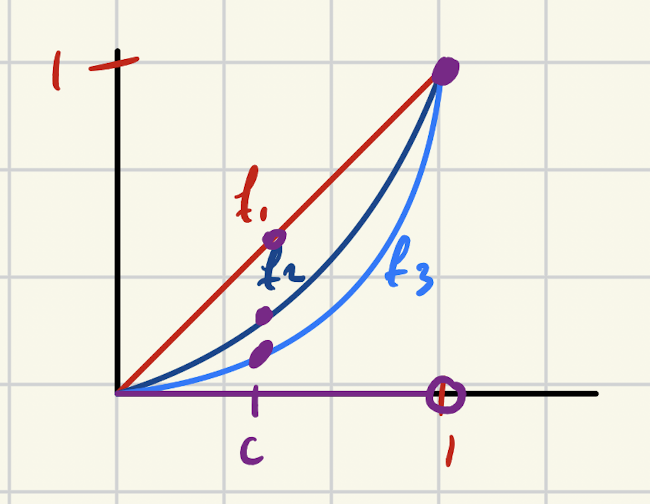
\includegraphics[width=0.25\textwidth]{CH7/images/Sequence of Functions c^n.png}
    \end{center}
\end{example}

\begin{observation}
    In this example, each $f_n$ is continuous but the pointwise limit $f$ is not continuous.
\end{observation}

\begin{remark}
    The pointwise limit of a sequence of continuous functions is not necessarily continuous.
    $$\text{"Pointwise convergence does not preserve convergence."}$$
\end{remark}

\begin{example}
    $\forall n \geq 1$ $f_n:[0,1] \to \R, f_n(x) = \begin{cases*}
        x & if $x \leq n$ \\
        n & if $x > n$
    \end{cases*}.$ Prove $f_n \to f$ pointwise where $f:[0,\infty) \to \R$ is defined by $f(x) = x.$

    At each point $c \in [0, \infty),$ the corresponding sequence of numbers is 
    $$(f_n(c))_{n\geq 1} = (f_1(c), f_2(c), f_3(c), ...).$$
    Note that for fixed $c \in [0, \infty),$ $\exists N \in \N \st c \leq N,$ so clearly
    $$c \leq N, ~~c \leq N+1, ~~c \leq N+2,...$$
    Thus
    $$f_N(c) = c, f_{N+1}(c) = c, f_{N+2}(c) = c, ...$$
    Therefore,
    $$(f_n(c))_{n \geq 1} = (f_1(c), f_2(c), f_3(c), ..., f_{N-1}(c), c, c, c, ...).$$
    We conclude that
    $$\lim_{n \to \infty}f_n(c) = c.$$

    \begin{center}
        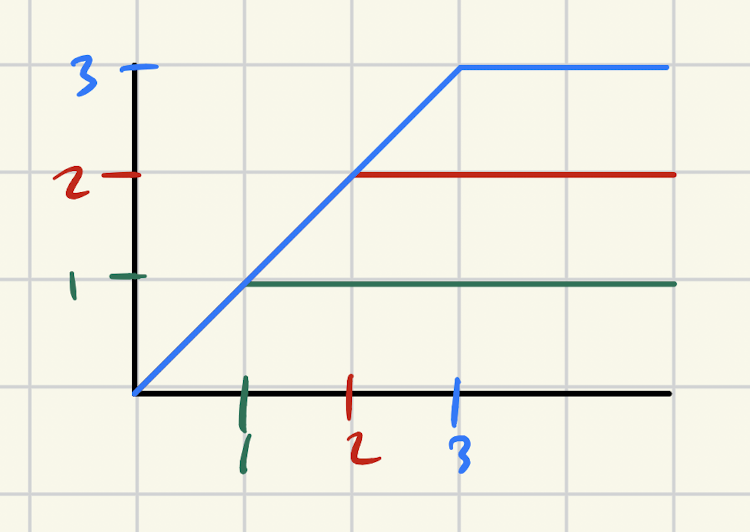
\includegraphics[width=0.25\textwidth]{CH7/images/Sequence of Bounded Functions.png}
    \end{center}
\end{example}

\begin{observation}
    Each $f_n$ is bounded, but $f(x) = x$ is not bounded.
\end{observation}

\begin{remark}
    The pointwise limit of a sequence of bounded functions is not necessarily bounded.
    $$\text{"Pointwise convergence does not preserve boundedness."}$$
\end{remark}

\begin{example}
    Let $f:[0,1] \to \R$ be a continuous, nowhere differentiable function. By the Weierstrass Approximation Theorem, there exists a sequence of polynomials $p_1(x), p_2(x), p_3(x),...$ such that $p_n$ converges to $f$ pointwise.
\end{example}

\begin{observation}
    Each $p_n$ is differentiable, but the pointwise limit $f$ is not differentiable.
\end{observation}

\begin{remark}
    The pointwise limit $f$ of a sequence of differentiable functions is not necessarily differentiable. Also, if $f'$ exists, it's not the case that $f_n' \to f'$.
    $$\text{"Pointwise convergence does not preserve differentiability."}$$
\end{remark}

\begin{example}
    $\forall n \geq 4,$ define $f_n:[0,1] \to \R$ as follows:
    $$f_n(x) = \begin{cases*}
        0 & if $0 \leq x < \frac{1}{n}$ \\
        n(nx-1) & if $\frac{1}{n} \leq x < \frac{2}{n}$ \\
        -n(nx-3) & if $\frac{2}{n} \leq x < \frac{3}{n}$ \\
        0 & if $\frac{3}{n} \leq x \leq 1$
    \end{cases*}.$$
    Prove that $f_n \to f$ pointwise where $f \equiv 0.$
    
    At each fixed point $c \in [0,1]$, the corresponding sequence of numbers
    $$(f_n(c))_{n \geq 4} = (f_4(c), f_5(c), f_6(c), ...).$$
    Note that
    \begin{align*}
        c = 0: ~~(f_n(0))_{n \geq 4} = (0,0,0,0,...) &\implies \lim_{n\to \infty}f_n(0) = 0 \\
        0 < c \leq 1: ~~ \exists N \in \N \st \frac{3}{N} < c &\implies \frac{3}{N} < c, \frac{3}{N+1} < c, \frac{3}{N+2} < c,... \\
        &\implies f_N(c) = 0, f_{N+1}(c) = 0, f_{N+2}(c) = 0, ... \\
        &\implies (f_n(c))_{n \geq 4} = (f_4(c), f_5(c), ..., f_{N-1}(c), 0, 0, ...) \\
        &\implies \lim_{n\to \infty}f_n(c) = 0.
    \end{align*}
    $\forall c \in [0,1],$ $\lim_{n\to \infty}f_n(c) = 0 = f(c)$, so $f_n \to f = 0$ pointwise.
\end{example}

\begin{observation}
    Each $f_n$, $\int_0^n f_n = 1$. However, $\int_0^1 f = 0$, so for every $n$ $\int_0^1 f_n \neq \int_0^1 f.$
\end{observation}

\begin{remark}
    Pointwise convergence does not allow us to interchange limits and integrals.
    $$\text{"Pointwise convergence does not preserve integrals."}$$
\end{remark}